

\chapter{Elektronik}
\label{chap:elektronik}

\section{Das Gehirn des Bootes}
Für die Steuerung des Bootes wird ein Raspberry Pi Zero W 1.1 verwendet. Dieser verfügt über ausreichend Leistung um alle notwendigen Berechnungen in Echtzeit durchzuführen. Auf dem Rasperry Pi läuft ein Debian basiertes GNU/Linux Betriebssystem. Im Kapitel Autonomie wird auf die Software jedoch genauer Eingeangen.

\begin{figure}[H] 
  \centering
    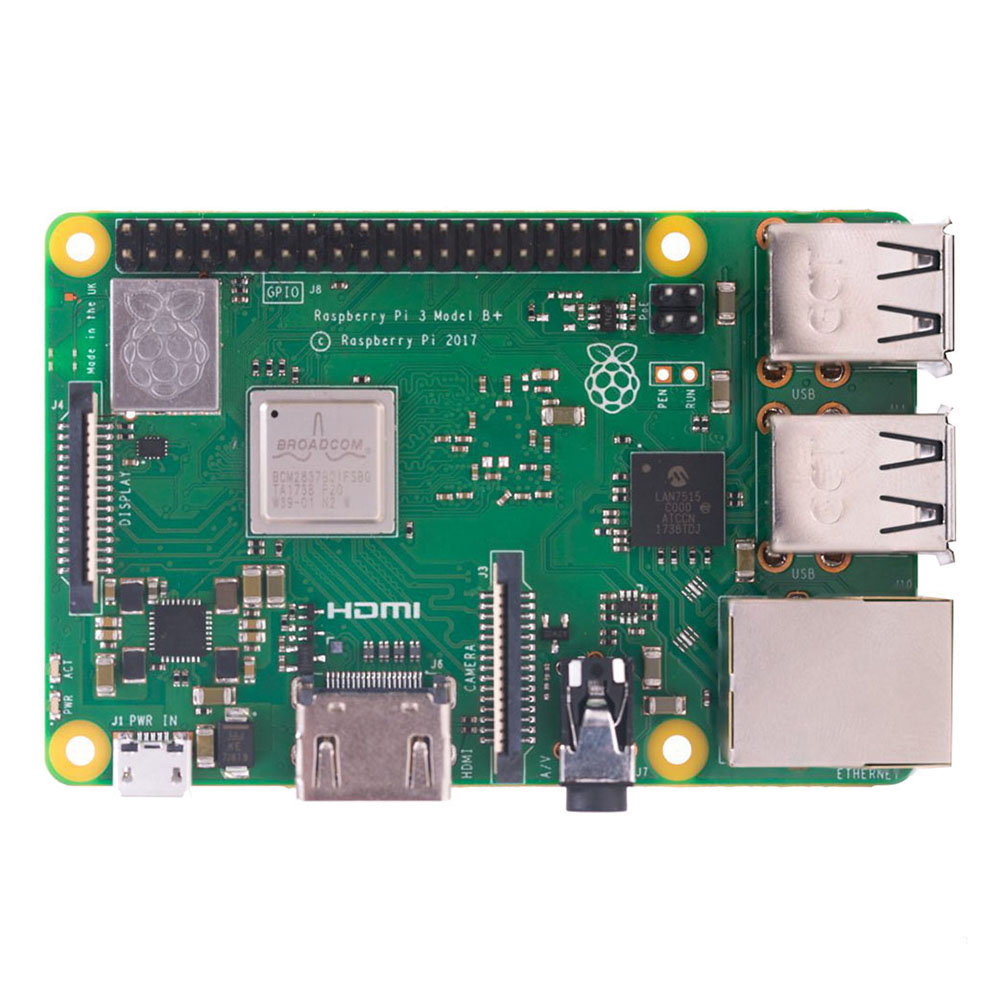
\includegraphics[width=0.5\linewidth]{PI_3B-plus-1-0.jpg}
    \caption{Raspberry 3 B+}
    \label{fig:rp3b+}
\end{figure}




\section{Sensoren und Aktuatoren}
\subsection{GPS}
Zur Bestimmung des aktuellen Standorts wird das Modul Neo 7M von Whadda verwendet. Dieses ist über eine Serielle Verbindung (RX und TX pins) verbunden.
\begin{figure}[H] 
    \centering
    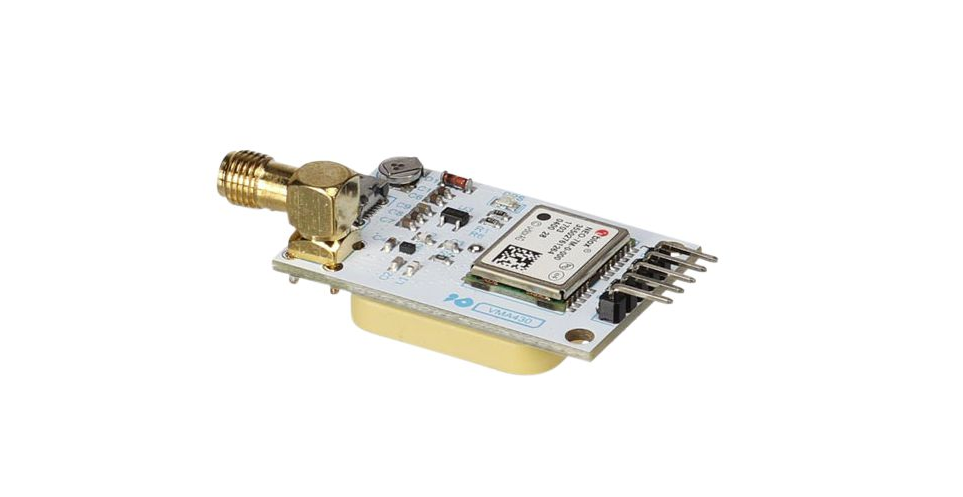
\includegraphics[width=0.5\linewidth]{gps.png}
    \caption{GPS Modul}
    \label{fig:gps}
\end{figure}

\subsection{Gyro und Magnetometer}
Kränung
\subsection{Aktuatoren}
Für die Bewegung der Elemente wurden L16-100-63-6-R Aktuatoren von Actuonix verwendet. Diese sind für den Robotik ausgelegt und Wasserdicht, was sie für diese Anwendung perfekt macht. Diese werden für das Ruder und das Segel verwendet. Mit 6V (und 5V) können sie betrieben werden und haben eine 63:1 Übersetzung. Dies macht sie nicht besonders schnell, jedoch erfüllen sie laut Hersteller die erforderliche Kraft.
Sie verfügen über kein Positionsfedback, sprich digital kann nicht abgefragt werden an welcher Position sich der "Stab" gerade befindet jedoch können konkrete Distanzen angesteuert werden. Verbunden wird der Aktuator mit dem einem Vcc und einer Ground Verbindung. Über eine einzige Datenverbindung können kurze Impulse zwischen 1ms-2ms gesendet werden, wobei 1ms die Startposition ist und der Aktuator bei 2ms voll ausgefahren wird. Um Einstellungen dazwischen zu erhalten, kann ein Wert zwischen 1ms und 2ms gesendet werden.  
\begin{figure}[H] 
    \centering
    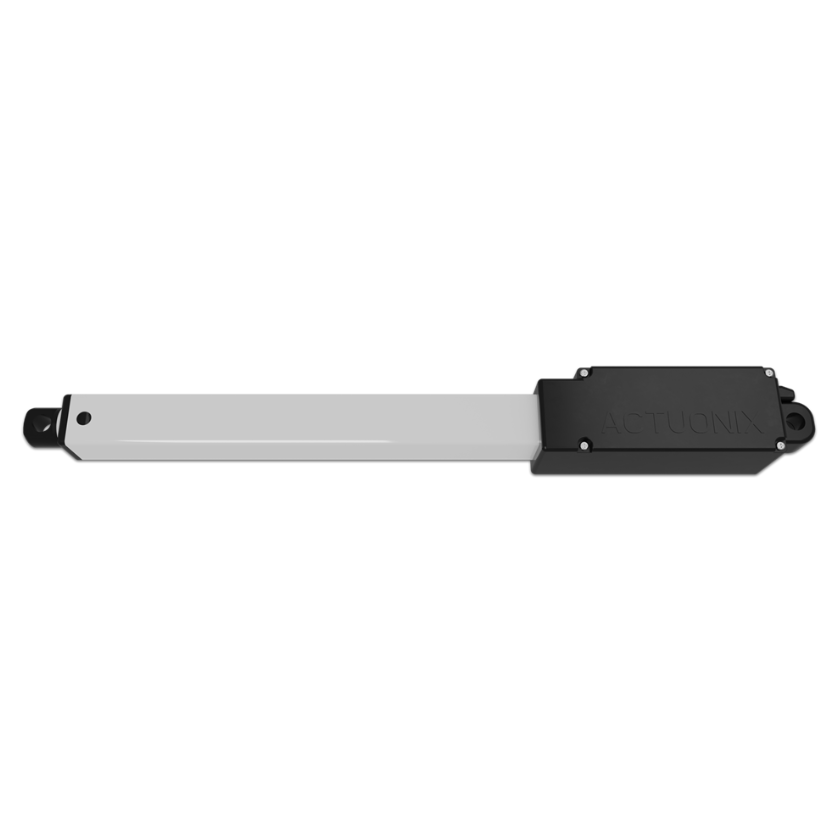
\includegraphics[width=0.5\linewidth]{actuonix.png}
    \caption{Actuonix Aktuator}
    \label{fig:actuator}
\end{figure}

\subsection{Kompass}
Um die Richtung 

\subsection{Windrichtungssensor}
Auf dem Markt gibt es erstaunlich wenige Windrichtungsmesser welche für dieses Projekt anwendbar wären. Manche sind zu gross, manche brauchen Energiemengen welche mir auf einem Boot nicht zur Verfügung stehen und wiederum andere sind schlichtweg zu teuer. Daher ist die entscheidung gefallen einen solchen, effizienteren jedoch möglichst kostengünstigen Sensor zu entwickeln.
Populär sind vorallem zwei typen von Windrichtungssensoren, welche eine unterschiedliche Angehensweise haben, die Richtung des Windes digital festzuhalten. \\
Zum einen wären das Sensoren welche mithilfe eines Pontiometer funktionieren. Diese sind mechanisch sehr leicht umzusetzen, da man lediglich einen kleinen flügel an einem Potentiometer befestigt. Die Position kann dann über einen Analogen Input pin auf einem Microcontroller eingelsen werden.
\\
Die zweite Option sind Hall Sensoren, mit welchen man typischerweise Stärke von Magneten misst. Um die Rotation eines Objektes mittels hallsensoren festzustellen gibt es 2 Möglichkeiten. Bei der ersten variante plaziert man um ein abwechselnd magnetisch positiv und magnetisch positiv geladenes rundes objekt eine belibige Anzahl an Hall sensoren um somit die Rotation zu messen. Jedoch ist es domit schwer einen genaue Position zu ermitteln zum einen aufgrund der Auflösung der Sensoren. 16 Sensoren bedeuten 360/16 grad akkuraität.  Die Zweite und deutlich veilversprechendere Option sind sogenannten Rotary Hall Sensors. Inmeinem Fall verwende ich einen AS5040-ASST mit einem Adapterbord um nicht smd (surface mount device) löten zu müssen, da es dieses Bauteil nicht als thd (through hole device) gibt. 

